% 原文 p.311
\hypertarget{srcpage:311}{}\label{srcpage:311}
一般の誤り演算子$\hat E_i$の重みは、構成要素である単一量子ビット演算子のうち、恒等演算子とは異なるものの個数と定義される。

幸い、量子誤り訂正に関係する多くの場合には、この一般的状況を簡単にしたものを使える。重要な場合の一つが、部分的デコヒーレンスである。ここでは、誤り訂正機構を二回適用するあいだに、少数の$K<N$個の量子ビットだけが環境ともつれる。この場合には、重みが$K$以下の$2^K$個の可能な誤り演算子だけに注意を限れば十分である。もう一つの重要な場合は、量子ビットの独立なデコヒーレンスである。ここでは重み1の誤り演算子だけに注目し、単一量子ビットに作用する独立な位相反転誤りの集まりを考える。したがって、各量子ビットは、他のすべての量子ビットとは独立に位相反転を受ける。位相反転誤りは複数の量子ビット間で相関せず、個々の量子ビットの場所で局所的にのみ起こる。独立な量子ビットのデコヒーレンスという仮定は、各量子ビットが主に自分自身の環境と結合し、これらの個別の環境が互いに相互作用しない状況で、物理的に正当化できる。たとえば、量子ビットが空間的に離れ、すぐ近くの周囲だけと結合する場合には、こうした状況になりうる。

\subsubsectionlink{量子コンピューターでデコヒーレンスを「取り消す」}
ここで上の結果と洞察を用いて、系に対するデコヒーレンスの影響を実効的に「取り消し」、量子ビット系をデコヒーレンス以前の元の状態へ戻すことで、量子誤り訂正をどう実現するかを見よう。系を測定して、どの誤りを訂正すべきかを調べ、系と環境を合わせたものを直接操作しようとする代わりに、アンシラと呼ばれる追加の量子ビット集合を用い、誤りの検出と訂正を助けてもらう。こうした補助量子ビットは、人工的な「環境」の役割を果たす。一般に、その物理的形態は計算用の量子ビットと同じだが、量子アルゴリズムの実際の実行には加わらない。その唯一の役割は、量子コンピューターがデコヒーレンスに対抗するのを助けることである。量子ビットと環境の系を操作する（不可能とまではいわなくても、難しい）代わりに、量子ビットとアンシラの系（これについては完全な制御が可能だと仮定する）に操作を行う。

量子ビット系Sとその環境Eのあいだの、もつれを生む相互作用の影響は、次の形で書けることを思い出そう。\footnote{ここではデコヒーレンスが引き起こす誤りに注目するが、以下の方式は任意の誤り演算子$\hat E_i$に成り立ち、$\hat Z_{j_1j_2\cdots j_N}$の形の誤り演算子に限られない。}［式(7.26)参照］
\begin{equation}|\psi\rangle|e_{\mathrm r}\rangle\longrightarrow\sum_i(\hat E_i|\psi\rangle)|e_i\rangle.\tag{7.30}\end{equation}
いまの目的は、式(7.30)右辺のもつれた状態が与えられたとき、初期状態$|\psi\rangle$（もちろん未知である！）を回復することである。
% 原文 p.312
\hypertarget{srcpage:312}{}\label{srcpage:312}
そのため、先に述べた補助量子ビット（以下ではAと書く）を導入しよう。これらの補助量子ビットの目的の一つは、次の意味で診断用の道具として働くことである。アンシラの初期状態が$|a_{\mathrm r}\rangle$で記述されるとしよう。ここでアンシラを量子ビット系と相互作用させ、
\begin{equation}|a_{\mathrm r}\rangle\left\{\sum_i(\hat E_i|\psi\rangle)|e_i\rangle\right\}\longrightarrow\sum_i|a_i\rangle(\hat E_i|\psi\rangle)|e_i\rangle\tag{7.31}\end{equation}
とする。この式は、アンシラが「装置」の役割を果たす、von Neumann型相互作用（2.5.1節参照）を記述する。以下の議論を明確にするため、式(7.31)右辺に現れるアンシラ状態$|a_i\rangle$は、少なくとも近似的に互いに直交し、そのため測定で区別できると仮定しよう。（この重要な問題は後で詳しく述べる。）

すると、次の手続きを用いられる（図7.2参照）。まず、アンシラについて可観測量
\begin{equation}\hat O_{\mathrm A}=\sum_i a_i|a_i\rangle\langle a_i|\tag{7.32}\end{equation}
を測定する。ただし$i\ne j$なら$a_i\ne a_j$である。この射影測定は、ある特定の結果、たとえば$a_k$を与え、式(7.31)右辺のもつれた状態を、重ね合わせの第$k$成分へ収縮させる。すなわち、
\begin{equation}\sum_i|a_i\rangle(\hat E_i|\psi\rangle)|e_i\rangle\longrightarrow|a_k\rangle(\hat E_k|\psi\rangle)|e_k\rangle.\tag{7.33}\end{equation}
測定結果が$a_k$であったことを知っているので、環境の影響を「取り消す」ために使う変換も、直ちにわかる。それは$\hat E_k^{-1}=\hat E_k^\dagger$である。（この特徴のために、補助量子ビットが「症状」$\hat E_k$の「診断道具」として働く、と先に述べたのである。）そこで量子ビット系に変換$\hat E_k^{-1}$を適用すると、
\begin{equation}|a_k\rangle(\hat E_k|\psi\rangle)|e_k\rangle\xrightarrow{\hat E_k^{-1}}|a_k\rangle|\psi\rangle|e_k\rangle\tag{7.34}\end{equation}
を得る。望む結果に到達した。量子ビットを元の状態$|\psi\rangle$へ戻すことに成功したのである。このようにして、実際にデコヒーレンスの有害な効果から回復した。

量子ビット系の計算基底で追加のデコヒーレンスを生じさせないために必要なとおり、量子ビット自体の状態については、いかなる情報も得ていないことに注意しよう。代わりに、複合量子ビット・環境系をアンシラと量子的に相関させることで、さまざまな誤り$\hat E_i$についての情報を、アンシラの異なる相対状態$|a_i\rangle$へ符号化した。アンシラの各状態$|a_i\rangle$は、誤り演算子$\hat E_i$によって変換されてはいるものの、量子ビットの完全な初期状態$|\psi\rangle$と相関しているので、量子ビットに含まれる量子情報を壊さずに、安全にアンシラを測定できる。
% 原文 p.313
\hypertarget{srcpage:313}{}\label{srcpage:313}
\begin{figure}[htbp]\centering
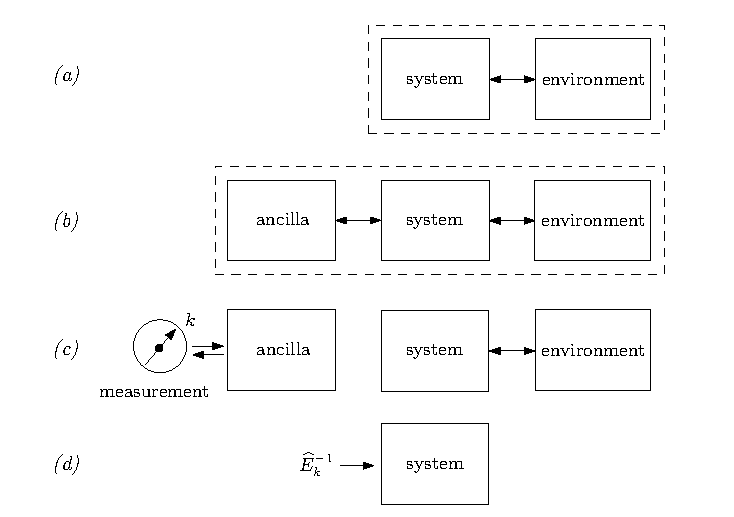
\includegraphics[width=.9\linewidth]{figures/ch07_fig02.pdf}
\caption{補助量子ビットによる量子誤り訂正。(a) 系Sと環境Eの相互作用によって、両者がもつれる［式(7.30)参照］。(b) 補助量子ビットAをSと相互作用させ、S、A、Eを含む三者もつれ状態(7.31)を作る。(c) Aへの射影測定が、この状態を式(7.33)の形の積状態へ収縮させ、実効的に部分系間のもつれを解く。測定結果には、訂正すべき誤りの情報が含まれる。(d) 適切な逆変換$\hat E_k^{-1}$の適用により、Sの元の状態が回復する。}
\end{figure}
するとアンシラの測定は、アンシラ・量子ビット・環境を合わせた全複合状態を、これらの誤りの一つに同時に収縮させ（系に、可能な誤りの集合$\{\hat E_i\}$から一つを「決める」よう「強制した」）、どの誤りが選び出されたかを教えてくれる。したがって、元の重ね合わせ状態を再構成する課題は、一つの既知の離散的誤り$\hat E_k$を反転することに帰着した。

この意味で、量子誤り訂正の基本的な考えは、Preskillの言葉を借りれば\cite{ref360}、「もつれをもってもつれに対抗する」ことである。この表現で伝えたいのは、量子ビットと環境を合わせた系を、私たちが完全に制御できる第三の「人工環境」、すなわちアンシラともつれさせれば、量子ビット系に対する環境もつれの有害な効果に対抗できる、という洞察である。誤り回復の手続きは、エントロピーを量子ビットからアンシラへ移した。したがってアンシラは、環境との相互作用によって量子ビット系に導入されたエントロピーの流しとして働く。
% 原文 p.314
\hypertarget{srcpage:314}{}\label{srcpage:314}
そのため、次の誤り訂正周期でアンシラを再利用する前に、補助量子ビットに保存された誤り情報をすべて「消去」しなければならない（すなわち、今度はアンシラを、別のエントロピーの流しへ結合しなければならない）。

上の量子誤り訂正の方式は、きわめて理想化されていた。とくに三つの問題が、実際の実現を難しくする。第一に、後の7.4.4節で論じるように、アンシラの測定によって可能な誤りすべてを区別できるような、計算用量子ビットとアンシラの相互作用を設計することは不可能である。第二に、現実的な状況では誤り演算子$\hat E_i$は非常に複雑かもしれない。対応する逆変換を、さらに大きなデコヒーレンスを加えることなく、量子コンピューターに適用できるか、どう適用するかは、なお検討を要する（その物理的実現には、計算用量子ビットと何らかの巨視的装置の相互作用が必要である）。第三に、補助量子ビットは計算用量子ビットと物理的に似ているため、計算用量子ビット自体と同じく環境との相互作用（したがってデコヒーレンス）を受けやすいと予想される。環境による補助量子ビットのこのような実効的測定は、量子誤り訂正方式の適切な動作を損なう。補助量子ビットを加えると量子コンピューター内の量子ビットの総数が増え、デコヒーレンス率は通常、系の大きさに対して指数関数的に増加するため、量子誤り訂正が実際に働くことだけでなく、意図せず量子ビットのデコヒーレンス問題をさらに悪化させないことも保証するには、精巧な実験設計が必要となる。

\subsubsectionlink{誤り訂正符号はいつ存在するか}
上の量子誤り訂正の基本原理の概説をできるだけ単純にするため、アンシラと量子ビットを合わせた系のHilbert空間に作用し、アンシラの相対状態$|a_i\rangle$がすべて区別可能で、異なる誤り型$\hat E_i$に対応するような、相関したアンシラ・量子ビット・環境状態を生むユニタリー変換が存在すると仮定した［式(7.31)参照］。すなわち、異なる二つの誤り$\hat E_i\ne\hat E_j$について$\langle a_i|a_j\rangle\approx\delta_{ij}$である。しかし、この変換が存在することをどう示し、どう決定するかという問いには、まったく立ち入らなかった。

実際、この問いは量子誤り訂正の核心にある。原理的に起こりうる、すべての誤り$\hat E_i$に対応する変換を見つけるのは、通常不可能であることがわかる。代わりに、量子誤り訂正方式が通常扱うのは、重みがある$t<N$以下であるすべての誤り$\hat E_i$を区別できる、式(7.31)の形の変換に限られる。さらに誤り訂正符号は通常、任意の初期量子ビット状態を回復できるわけではなく、量子ビット系の全Hilbert空間$\mathcal H_{\mathrm S}$の、ある部分空間$\mathcal H_{\mathrm{code}}$に含まれる状態だけを回復できる。
% 原文 p.315
\hypertarget{srcpage:315}{}\label{srcpage:315}
（部分空間$\mathcal H_{\mathrm{code}}$は、その量子誤り訂正方式の符号部分空間とよく呼ばれる。）

上の概説で見たように、量子誤り訂正の基本的方策は、誤り演算子$\hat E_i$で区別される直交部分空間へ、量子ビット状態を射影することである。そうすれば、これらの誤り部分空間のどれへ状態が射影されたかを明らかにする測定を行え、誤りを訂正するためにどの逆変換を使うかという情報を得られる。したがって形式的には、ある重み$t$までの誤りを訂正できる誤り訂正符号が存在するための十分条件（必要条件ではない）は、「誤りによって射影された」部分空間
\begin{equation}\{\hat E_i\mathcal H_{\mathrm{code}}\mid\operatorname{weight}(\hat E_i)\leq t\}\tag{7.35}\end{equation}
が、すべての$i$について（少なくとも近似的に）互いに直交することを要求することで与えられる。すると任意の初期状態$|\psi\rangle\in\mathcal H_{\mathrm{code}}$に対し、擾乱後の状態の展開に現れる異なる誤り項$\hat E_i|\psi\rangle|e_i\rangle$は互いに直交し、そのため、状態$|\psi\rangle$自体に符号化された量子情報を明らかにせずに、測定で区別できる。

\subsubsectionlink{冗長符号化の重要性と位相誤りのための三ビット符号}
条件(7.35)を満たすには、通常、冗長符号化を使う必要があることがわかる。7.4.1節では、古典計算で冗長符号化が、擾乱を受ける前の元の状態の回復にどう役立つかを説明した。また、未知の量子状態を複製できないことも述べた。しかし式(7.14)は、計算基底状態を優先基底として用い、「相対状態」の形で冗長符号化を容易に行う方法を示していることに注意しよう。すなわち、第一の量子ビットと、他のすべての量子ビットとのあいだに、CNOTゲートの列を単に適用すればよい。
\begin{equation}(\alpha|0\rangle+\beta|1\rangle)|00\cdots0\rangle\longrightarrow\alpha|000\cdots0\rangle+\beta|111\cdots1\rangle.\tag{7.36}\end{equation}
このような冗長符号化は、量子誤りの訂正にどう役立つのだろうか。

まず、こうした符号化なしには通常あまり先へ進めない理由を見るため、単一量子ビット状態$|\psi\rangle=\alpha|0\rangle+\beta|1\rangle$が環境ともつれる例を考えよう。最終的な複合状態は、次のように書ける［式(7.24)参照］。
\begin{equation}|\Psi\rangle=\frac1{\sqrt2}[(\alpha|0\rangle+\beta|1\rangle)|e_+\rangle+(\alpha|0\rangle-\beta|1\rangle)|e_-\rangle].\tag{7.37}\end{equation}
式(7.31)に含まれる仮定は、二つの直交するアンシラ状態$|a_0\rangle$と$|a_1\rangle$、およびアンシラと量子ビットを合わせた系のHilbert空間に作用するユニタリー変換が存在し、時間発展
% 原文 p.316
\hypertarget{srcpage:316}{}\label{srcpage:316}
\begin{equation}\begin{aligned}|a_{\mathrm r}\rangle|\Psi\rangle\longrightarrow\frac1{\sqrt2}\big[&|a_0\rangle(\alpha|0\rangle+\beta|1\rangle)|e_+\rangle\\+&|a_1\rangle(\alpha|0\rangle-\beta|1\rangle)|e_-\rangle\big]\end{aligned}\tag{7.38}\end{equation}
を起こせるというものである。しかし$\beta\longrightarrow-\beta$と置き換えると、「誤りの指標」としてのアンシラ状態の役割は逆転する。すなわち、今度はアンシラ状態$|a_0\rangle$が位相反転型の項と相関し、$|a_1\rangle$は誤りのない項に対応する。したがって、アンシラを測定しても、生じた誤りについて有益な情報は得られない。ただしもちろん、係数$\alpha$と$\beta$について何かを知っている場合（そして、それに応じてアンシラ状態がこれらの係数の何らかの関数である場合）は別である。しかし初期量子ビット状態は一般に完全に未知なので、このような知識があるとは明らかに仮定できない。\footnote{これはもちろん、古典的な場合にも量子的な場合にも、誤り訂正の眼目そのものである。擾乱された状態が与えられ、未知の初期状態を再構成したいのである。擾乱されていない状態が何であるべきかを最初から知っていれば、単に系をその状態へ準備し直すだけで自明に済む。}

この困難は、量子誤り訂正が、より単純な量子「消去」の方法（2.13節参照）と異なることを示す。式(7.37)と(7.38)が記述する時間発展は、本質的に「消去」手順(2.125)のものであり、アンシラと環境がそれぞれ読み出し装置と経路検出器に対応することに注意しよう。量子「消去」では、読み出し測定(2.124)の結果を、スクリーン上で観測された粒子の位置に条件付けるという意味で、干渉縞が回復される\cite{ref130}。この条件付けが必要なのは、式(2.125)の状態$|\psi_+\rangle$と$|\psi_-\rangle$が、それぞれスクリーン上の縞と「反縞」のパターンに対応し、それらを合わせたパターンは、干渉のない古典分布に等しくなるためである。したがって、干渉縞の実効的回復には、読み出し装置の最終的な相対状態$|\Phi_\pm\rangle$を区別できることが必要だが、状態$|\psi_\pm\rangle$の中の成分$|\psi_1\rangle$と$|\psi_1\rangle$の相対位相の具体的な値を、読み出し測定から推定する必要はない。これに対して量子計算では、元の重ね合わせ状態を回復することが重要である。したがって、計算基底状態間の相対位相を検出し、訂正できる必要があるが、式(7.38)はこの要求を満たさない。

この問題は、単一量子ビット状態を冗長に符号化することで解決できる。この方法を説明するため、方式(7.36)を用い、一つの論理量子ビットを三つの物理量子ビットへ冗長に符号化する例を考えよう。
\begin{equation}(\alpha|0\rangle+\beta|1\rangle)|00\rangle\longrightarrow\alpha|000\rangle+\beta|111\rangle.\tag{7.39}\end{equation}
以下で見るように、この符号化により、初期量子ビット状態をまったく知らなくても、一つの量子ビットに影響する位相反転誤りを診断し（そして回復する）ことが可能になる。

まず、符号化された状態(7.39)を、各量子ビットについて共役基底$\{|+\rangle,|-\rangle\}$へ変換する。ここで$|\pm\rangle=(|0\rangle\pm|1\rangle)/\sqrt2$である。
